% Options for packages loaded elsewhere
\PassOptionsToPackage{unicode}{hyperref}
\PassOptionsToPackage{hyphens}{url}
%
\documentclass[
]{article}
\usepackage{lmodern}
\usepackage{amssymb,amsmath}
\usepackage{ifxetex,ifluatex}
\ifnum 0\ifxetex 1\fi\ifluatex 1\fi=0 % if pdftex
  \usepackage[T1]{fontenc}
  \usepackage[utf8]{inputenc}
  \usepackage{textcomp} % provide euro and other symbols
\else % if luatex or xetex
  \usepackage{unicode-math}
  \defaultfontfeatures{Scale=MatchLowercase}
  \defaultfontfeatures[\rmfamily]{Ligatures=TeX,Scale=1}
\fi
% Use upquote if available, for straight quotes in verbatim environments
\IfFileExists{upquote.sty}{\usepackage{upquote}}{}
\IfFileExists{microtype.sty}{% use microtype if available
  \usepackage[]{microtype}
  \UseMicrotypeSet[protrusion]{basicmath} % disable protrusion for tt fonts
}{}
\makeatletter
\@ifundefined{KOMAClassName}{% if non-KOMA class
  \IfFileExists{parskip.sty}{%
    \usepackage{parskip}
  }{% else
    \setlength{\parindent}{0pt}
    \setlength{\parskip}{6pt plus 2pt minus 1pt}}
}{% if KOMA class
  \KOMAoptions{parskip=half}}
\makeatother
\usepackage{xcolor}
\IfFileExists{xurl.sty}{\usepackage{xurl}}{} % add URL line breaks if available
\IfFileExists{bookmark.sty}{\usepackage{bookmark}}{\usepackage{hyperref}}
\hypersetup{
  hidelinks,
  pdfcreator={LaTeX via pandoc}}
\urlstyle{same} % disable monospaced font for URLs
\usepackage{graphicx}
\makeatletter
\def\maxwidth{\ifdim\Gin@nat@width>\linewidth\linewidth\else\Gin@nat@width\fi}
\def\maxheight{\ifdim\Gin@nat@height>\textheight\textheight\else\Gin@nat@height\fi}
\makeatother
% Scale images if necessary, so that they will not overflow the page
% margins by default, and it is still possible to overwrite the defaults
% using explicit options in \includegraphics[width, height, ...]{}
\setkeys{Gin}{width=\maxwidth,height=\maxheight,keepaspectratio}
% Set default figure placement to htbp
\makeatletter
\def\fps@figure{htbp}
\makeatother
\setlength{\emergencystretch}{3em} % prevent overfull lines
\providecommand{\tightlist}{%
  \setlength{\itemsep}{0pt}\setlength{\parskip}{0pt}}
\setcounter{secnumdepth}{-\maxdimen} % remove section numbering
\usepackage{epsdice}
\ifluatex
  \usepackage{selnolig}  % disable illegal ligatures
\fi

\author{}
\date{}

\begin{document}

\hypertarget{probability-basics}{%
\section{Probability Basics}\label{probability-basics}}

\hypertarget{outcomes-and-sample-space}{%
\section{Outcomes and Sample Space}\label{outcomes-and-sample-space}}

Probability begins with a set \(X\) of ``outcomes''. This set may be
continuous or discrete.

\begin{itemize}
\item
  \(X=\{H,T\}\), the result of a single coin flip. (discrete)
\item
  \(X\) is the possible results of throwing two six-sided dice --
  ordered pairs. (discrete)
\item
  \(X\) is the set of real numbers, where a value \(x\) means measuring
  the temperature \(t_0+x\) where \(t_0\) is the ``true'' temperature.
  (continous)
\end{itemize}

The set \(X\) of possible outcomes is called the \emph{sample space.}

\hypertarget{event}{%
\section{Event}\label{event}}

An ``event'' is a subset of the sample space -- a collection of
outcomes.

The probability function \(P\) takes values between \(0\) and \(1\) and
measures the ``chance'' that an event ``occurs.''

If a sequence of events are disjoint, then the probability of them all
happening is the sum of their probabilities.

\[
P(U_1\cup\cdots\cup U_n)=\sum_{i=1}^{n} P(U_i)
\]

\hypertarget{events---discrete-examples}{%
\section{Events - discrete examples}\label{events---discrete-examples}}

\begin{itemize}
\item
  \(P(\{H\})=1/2\)
\item
  \$P(\{(\epsdice{1},\epsdice{5})\}) = 1/36
\item
  the probability of the event \(E\) consisting of throwing two dice
  that sum to 5: \[
  E=\{(\epsdice{1},\epsdice{4}),(\epsdice{2},\epsdice{3}),(\epsdice{3},\epsdice{2}),(\epsdice{4},\epsdice{1})\}
  \] is \((4)(1/36)=1/9\)
\end{itemize}

\hypertarget{events---continuous-example}{%
\section{Events - continuous
example}\label{events---continuous-example}}

\begin{itemize}
\item
  \(X=\mathbf{R}\).
\item
  Probability arises from a density function \(p(x)\)
\item
  \(P(U) = \int_{U} p(x)dx\)
\item
  \(\int_{-\infty}^{\infty}p(x)dx=1\).
\end{itemize}

\hypertarget{normal-distribution}{%
\section{Normal distribution}\label{normal-distribution}}

\begin{itemize}
\item
  Measure temperature \(t\) using a thermometer.
\item
  True temperature is \(t_{0}\).
\item
  Error \(x=t-t_{0}\) \[
  P(|t-t_{0}|<\delta) =\int_{x=-\delta}^{\delta} p_{\sigma}(x)dx
  \] where \[
  p_{\sigma}(x) = \frac{1}{\sigma\sqrt{2\pi}}e^{-x^2/(2\sigma^2)}.
  \]
\end{itemize}

\(\sigma\) is called the ``standard deviation''.

\hypertarget{normal-distribution-contd}{%
\section{Normal distribution cont'd}\label{normal-distribution-contd}}

\begin{figure}
\centering
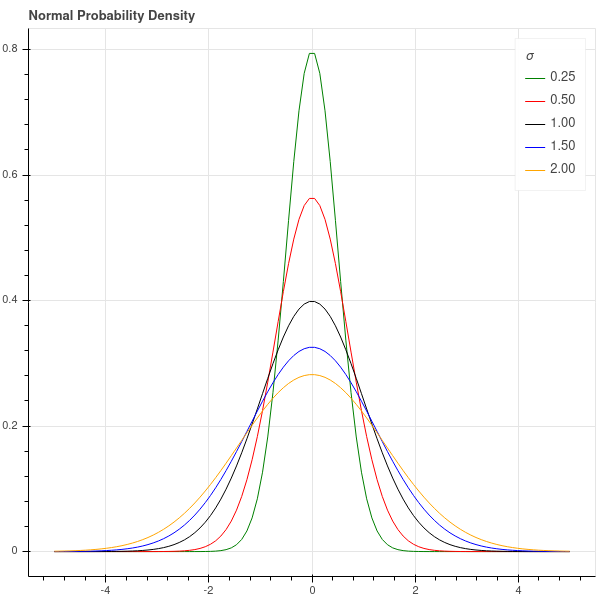
\includegraphics[width=0.7\textwidth,height=\textheight]{../img/density.png}
\caption{Normal Distributions}
\end{figure}

\end{document}
